%%%%%%%%%%%%%%%%%%%%%%%%%%%%%%%%%%%%%%%%%%%%%%%%%%%%%%%%%%%%%%%%%%%%%%
% CAPA DO PROJETO DE DISSERTA??O
%%%%%%%%%%%%%%%%%%%%%%%%%%%%%%%%%%%%%%%%%%%%%%%%%%%%%%%%%%%%%%%%%%%%%%

\thispagestyle{empty}

\begin{center}

\begin{minipage}[b]{0.2\linewidth}
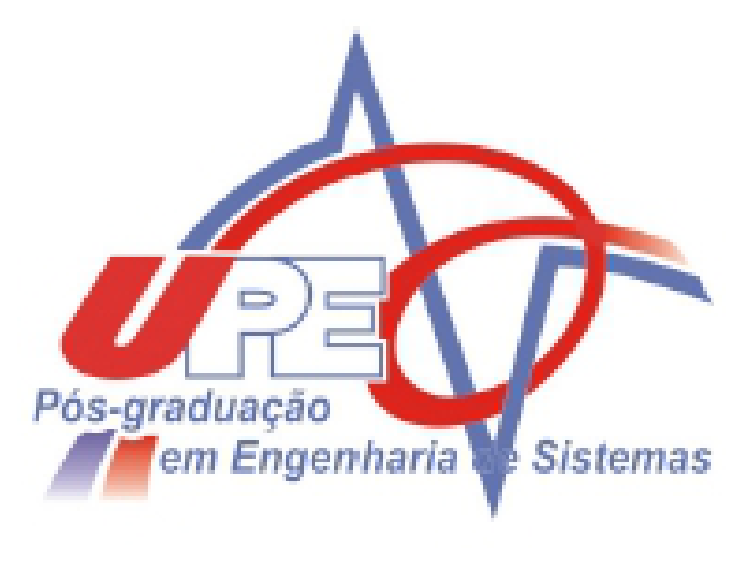
\includegraphics[width=\textwidth]{Figuras/Capa/logo_ppges.eps}
\end{minipage} \hfill
\begin{minipage}[b]{0.15\linewidth}

\includegraphics[width=\textwidth]{Figuras/Capa/brasao_upe.eps}
\end{minipage} \hfill
\begin{minipage}[b]{0.2\linewidth}

\includegraphics[width=\textwidth]{Figuras/Capa/upelogo.eps}
\end{minipage}

%==(CABE?ALHO)========================================================
{\textbf{Universidade de Pernambuco (UPE)}}% \\ \vspace{1ex}

{\textbf{Escola Politécnica de Pernambuco (POLI)}}%\\ \vspace{1ex}

{\textbf{Instituto de Ciências Biológicas (ICB)}} \\ \vspace{2ex}

{\textbf{Programa de Pós-Graduação em Engenharia de Sistemas}} \\ \vspace{1ex}
%=====================================================================

\vspace{0.8in}

{\Large Hugo Abreu Mendes}\\

\vspace{1in}

%===(T?TULO DO PROJETO DE DISSERTA??O)================================
{\Large \textbf{MODELOS HÍBRIDOS AUTOMATIZADOS PARA PREVISÃO DE IRRADIAÇÃO SOLAR}} \\
%=====================================================================

\vspace{0.3in}

%===(NOME DO ALUNO E DO ORIENTADOR)===================================

%\vspace{1ex} {\textbf{Orientador: Prof$^{a}$. Dr$^{a}$. Maria de Lourdes Melo Guedes Alcoforado} }

%=====================================================================

\end{center}

%===(IDENTIFICADOR DO DOCUMENTO)===================================
\begin{flushright}
    \vspace{0.5in}
    \parbox{3.50in}
    %{\textbf{Dissertação} apresentada à Universidade de Pernambuco como parte dos %requisitos para a obtenção do título de Mestre em Engenharia de Sistemas.
    %\\ 
    %\\Área de concentração: \textbf{Telemática} 
    %}
    {\textbf{Projeto de Mestrado} redigido para o Programa de Pós-Graduação em Engenharia de Sistemas, como parte dos requisitos para defesa de dissertação.
    }

\end{flushright}
%===================================================================

\vspace{1.2ex}

\begin{center}

%===(IDENTIFICA??O DA BANCA DE QUALIFICA??O E DATA(M?S/ANO))========


\vspace{1ex} {\textbf{Orientadora: Prof. Dr. Manoel Henrique da Nóbrega Marinho} }\\
\vspace{1ex} {\textbf{Coorientador: Prof. Dr. João Fausto Lorenzato de Oliveira} }


\vspace{0.2in}
\vspace{18pt}{Recife, Março de 2021.}
%==================================================================

\end{center}

